\section{Frequenzverhalten \formelbuch{205-251}}
\subsection{Logarithmische Darstellung \formelbuch{206-210}}
\begin{tabular}{ll}
\parbox{7cm}{
	\scriptsize
	\begin{tabular}{|c|c|c|c|}
	\hline
	\textbf{Lrel. (dB)} & \textbf{Lrel. (NP)} & \textbf{P2/P1} & \textbf{A2/A1} \\ \hline
	$100.000$ & $11.513$ & $10^{10}$ & $10^5$ \\ \hline
	$90.000$ & $10.362$ & $10^9$ & $31622.777$ \\ \hline
	$80.000$ & $9.210$ & $10^8$ & $10^4$ \\ \hline
	$70.000$ & $8.059$ & $10^7$ & $3162.278$ \\ \hline
	$60.000$ & $6.908$ & $10^6$ & $10^3$ \\ \hline
	$50.000$ & $5.756$ & $10^5$ & $316.228$ \\ \hline
	$40.000$ & $4.605$ & $10^4$ & $10^2$ \\ \hline
	$30.000$ & $3.454$ & $10^3$ & $31.623$ \\ \hline
	\textbf{$20.000$} & $2.303$ & \textbf{$10^2$} & \textbf{$10.000$} \\ \hline
	$19.085$ & $2.197$ & $81.000$ & $9.000$ \\ \hline
	$19.000$ & $2.187$ & $79.433$ & $8.913$ \\ \hline
	$18.062$ & $2.079$ & $64.000$ & $8.000$ \\ \hline
	$18.000$ & $2.072$ & $63.096$ & $7.943$ \\ \hline
	$17.000$ & $1.957$ & $50.119$ & $7.079$ \\ \hline
	$16.902$ & $1.946$ & $49.000$ & $7.000$ \\ \hline
	$16.000$ & $1.842$ & $39.811$ & $6.310$ \\ \hline
	$15.563$ & $1.792$ & $36.000$ & $6.000$ \\ \hline
	$15.000$ & $1.727$ & $31.623$ & $5.623$ \\ \hline
	$14.000$ & $1.612$ & $25.119$ & $5.012$ \\ \hline
	\textbf{$13.979$} & $1.609$ & \textbf{$25.000$} & \textbf{$5.000$} \\ \hline
	$13.000$ & $1.497$ & $19.953$ & $4.467$ \\ \hline
	\textbf{$12.041$} & $1.386$ & \textbf{$16.000$} & \textbf{$4.000$} \\ \hline
	\textbf{$12.000$} & $1.382$ & $15.849$ & $3.981$ \\ \hline
	$11.000$ & $1.266$ & $12.589$ & $3.548$ \\ \hline
	\textbf{$10.000$} & $1.151$ & \textbf{$10.000$} & $3.162$ \\ \hline
	$9.542$ & $1.099$ & $9.000$ & $3.000$ \\ \hline
	$9.000$ & $1.036$ & $7.943$ & $2.818$ \\ \hline
	$8.000$ & $0.921$ & $6.310$ & $2.512$ \\ \hline
	$7.000$ & $0.806$ & $5.012$ & $2.239$ \\ \hline
	\textbf{$6.021$} & \textbf{$0.693$} & \textbf{$4.000$} & \textbf{$2.000$} \\ \hline
	$6.000$ & $0.691$ & $3.981$ & $1.995$ \\ \hline
	$5.000$ & $0.576$ & $3.162$ & $1.778$ \\ \hline
	$4.000$ & $0.461$ & $2.512$ & $1.585$ \\ \hline
	\textbf{$3.010$} & \textbf{$0.347$} & \textbf{$2.000$} & \textbf{$1.414$} \\ \hline
	$3.000$ & $0.345$ & $1.995$ & $1.413$ \\ \hline
	$2.000$ & $0.230$ & $1.585$ & $1.259$ \\ \hline
	$1.000$ & $0.115$ & $1.259$ & $1.122$ \\ \hline
	$0.000$ & $0.000$ & $1.000$ & $1.000$ \\ \hline
	-$1.000$ & -$0.115$ & $0.794$ & $0.891$ \\ \hline
	-$2.000$ & -$0.230$ & $0.631$ & $0.794$ \\ \hline
	-$3.000$ & -$0.345$ & $0.501$ & $0.708$ \\ \hline
	-$4.000$ & -$0.461$ & $0.398$ & $0.631$ \\ \hline
	-$5.000$ & -$0.576$ & $0.316$ & $0.562$ \\ \hline
	-$6.000$ & -$0.691$ & $0.251$ & $0.501$ \\ \hline
	-$7.000$ & -$0.806$ & $0.200$ & $0.447$ \\ \hline
	-$8.000$ & -$0.921$ & $0.158$ & $0.398$ \\ \hline
	-$9.000$ & -$1.036$ & $0.126$ & $0.355$ \\ \hline
	-$10.000$ & -$1.151$ & $0.100$ & $0.316$ \\ \hline
	-$15.000$ & -$1.727$ & $0.032$ & $0.178$ \\ \hline
	-$20.000$ & -$2.303$ & $10^{-2}$ & $0.100$ \\ \hline
	-$30.000$ & -$3.454$ & $10^{-3}$ & $0.032$ \\ \hline
	-$40.000$ & -$4.605$ & $10^{-4}$ & $0.010$ \\ \hline
	-$50.000$ & -$5.756$ & $10^{-5}$ & $0.003$ \\ \hline
	-$60.000$ & -$6.908$ & $10^{-6}$ & $0.001$ \\ \hline
	\end{tabular}
}
& \parbox{11.5cm}{
	\scriptsize
	\begin{tabular}{|c|c|c|c|}
	\hline
	-$70.000$ & -$8.059$ & $10^{-7}$ & $0.000$ \\ \hline
	-$80.000$ & -$9.210$ & $10^{-8}$ & $10^{-4}$ \\ \hline
	-$90.000$ & -$10.362$ & $10^{-9}$ & $3.162 \cdot 10^{-5}$ \\ \hline
	-$100.000$ & -$11.513$ & $10^{-10}$ & $10^{-5}$ \\ \hline
	\end{tabular} \\
	\normalsize
Verstärkungsmass L in \textbf{Dezibel} (dB):\\
$L_P = 10 \cdot \log \left(\frac {P_2} {P_1}\right) \qquad$ Index P: Leistung \\
$L_A = 20 \cdot \log \left(\frac {A_2} {A_1}\right) \qquad$ Index A: Amplitude \\ 

Dezibel L zu linear: \\
$P_2 = P_1 \cdot 10^{\frac{L_P}{10}} $ \\
$A_2 = A_1 \cdot 10^{\frac{L_A}{20}} $ \\

Verstärkungsmass L in \textbf{Neper} (Np):\\
$L_P = \frac {1}{2} \cdot \ln \left(\frac {P_2} {P_1}\right)$\\
$L_A = \ln \left(\frac {A_2} {A_1} \right)$ \\

Neper zu linear: \\
$P_2 = P_1 \cdot e^{2 L_P}$ \\
$A_2 = A_1 \cdot e^{L_A}$ \\

Die Umrechnung zwischen {\bf dB} und {\bf Np} ist linear: \\
$1\mbox{~dB} = \frac {\ln(10)} {20} \mbox{~Np} = 0.1151\mbox{~Np}$ \\
$1\mbox{~Np} = 20 \cdot \log(\mbox{e}) \mbox{~dB} = 8.686\mbox{~dB}$ \\ 
\\
Anstatt $\frac{X_2}{X_1}$ für Verstärkungsmasse ($L$) können auch
$\frac{X_1}{X_2}$ für \textbf{Dämpfungsmasse ($\bf{a}$)} verwendet werden!

\small{($P$ für Leistungen, $A$ für Amplituden)}
\\ 

\textbf{Hilfen zur Berechnung}\\
\begin{tabular}{|l|ll|}
\hline
$x dB$	& $T_P=P_2/P_1$ &$T_A=A_2/A_1$ \\
\hline
$-x dB$	& $1/T_P = D_P$	& $1/T_A = D_A$\\
$x+3dB$	& $T_P \cdot 2$	& $T_A \cdot \sqrt{2} \approx T_A \cdot 1.414$ \\
$x+6dB$ & $T_P \cdot 4$ & $T_A \cdot 2$ \\
$x+10dB$	& $T_P \cdot 10$ & $T_A \cdot \sqrt{10} \approx T_A \cdot 3.162$\\
\hline
\end{tabular}
\begin{tabular}{lllll}
  $T$: & Verstärkungsfaktor & &
  $D$: & Dämpfungsfaktor
\end{tabular}
\\ \\

\textbf{Relative Pegel}\\
\begin{tabular}{|l|l|}
  \hline
    dBu & Spannungspegel bezogen auf 774.6~mV (1~mW an $600\Omega$)\\
  \hline
  \hline
    dBV & Spannungspegel bezogen auf 1~V\\
  \hline
    dB$\mu$V & Spannungspegel bezogen auf 1~$\mu$V\\
  \hline
    dBW & Leistungspegel bezogen auf 1~W\\
  \hline
    dBm & Leistungspegel bezogen auf 1~mW\\
  \hline
\end{tabular}

}
\end{tabular}
\newpage

\subsection{Frequenzgang \formelbuch{211-219}}
\label{Polfrequenz Polguete}
  \begin{minipage}[l]{12cm}
    \[ H(s) = \frac{Y(s)}{X(s)}=\frac{b_ms^m+b_{m-1}s^{m-1}+\ldots+b_1s+b_0}
    {a_ns^n+a_{n-1}s^{n-1}+\ldots+a_1s+a_0} = \frac{N(s)}{D(s)}\]
    \[ H(s) = K \cdot \frac{\overbrace{\prod\limits_{i=1}^r(s^2+2\sigma_{zi}s+\omega_{zi}^2)}^{komplex}
    \overbrace{\prod\limits_{i=2r+1}^m (s-z_i)}^{reell}}{\prod\limits_{j=1}^t(s^2+2\sigma_{pj}s+\omega_{pj}^2)
    \prod\limits_{j=2t+1}^n(s-p_j)} \] 
    
    \begin{tabular}{|l|ll|}
      \hline
        Polfrequenz: 
          & $ \omega_p = \sqrt{\sigma_p^2+\tilde{\omega}_p^2}$ & (konj. komplexe Pole)\\
          & $\omega_p = \sqrt{\sigma_{p1} \cdot \sigma_{p2}}$ & (reelle Pole) \\
      \hline
        Polgüte: 
          & $ q_p = \dfrac{\omega_p}{2\cdot\sigma_p} = \dfrac{1}{2\cdot\cos\alpha} $ & (konj. komplexe Pole)\\
          & $q_p = \dfrac{\sqrt{\sigma_{p1} \cdot \sigma_{p2}}}{\sigma_{p1} + \sigma_{p2}} \leq \frac{1}{2}$ &
          (reelle Pole) \\
      \hline
    \end{tabular}
  \end{minipage}
  \begin{minipage}[c]{6cm}
    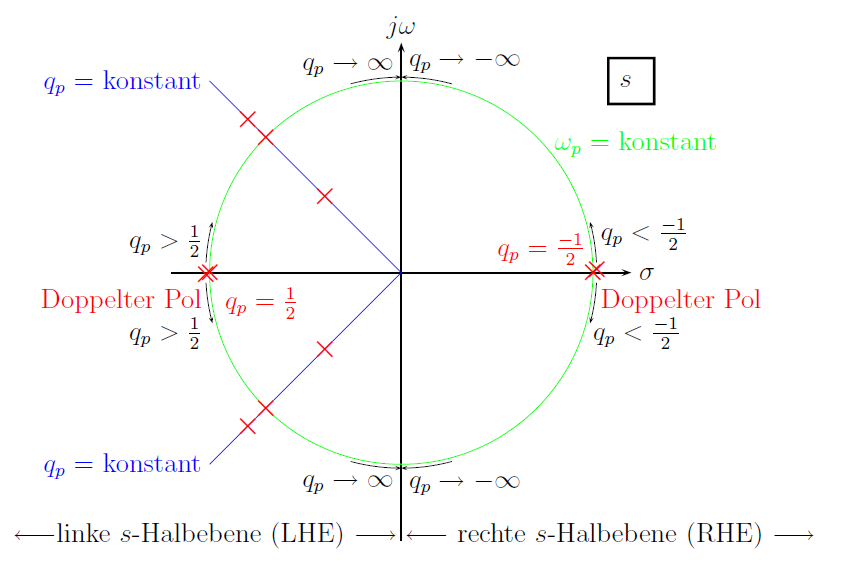
\includegraphics[width=6cm]{./images/FG_Pollage.png} \\
    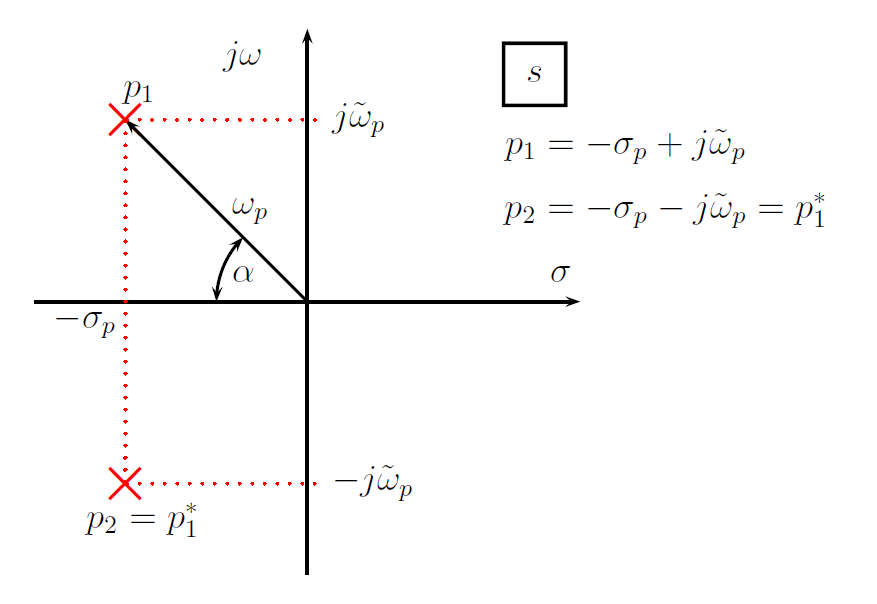
\includegraphics[width=6cm]{./images/FG_geoDeutung.png}
  \end{minipage}
  
  Für die \textbf{Nullstellen} gelten die gleichen geometrischen Beziehungen.
  Für einen \textbf{Einzelpol} ist die Güte nicht definiert! Die Polfrequenz entspricht dann dem Abstand zum Ursprung.
  
  \subsubsection{Bode-Diagramm und Pol-Nullstellenverteilung}
  siehe im Anhang

\subsection{Minimal- und nicht-minimalphasige Systeme \formelbuch{220-224}}
\subsubsection{Allpass-Systeme\formelbuch{220}}
Allpässe werden vor allem als Laufzeitkorrekturglieder und als
Verzögerungselemente verwendet. Der Amplitudengang ist konstant ($|H(jw)| =
const \neq 0$) und die Pol- bzw. Nullstellen haben in Paaren auftretende Null-
und Polstellen, die symmetrisch zur $j \omega$-Achse liegen. Dabei liegen die
Nullstellen auf der RHE.
UTF: $H_A(s) = K \frac{Q(-s)}{Q(s)}$ \\
Wobei $Q(s)$ ein striktes Hurwitz-Polynom ist.



\subsubsection{Minimalphasennetzwerke \formelbuch{221}}
\begin{itemize}
  \item Keine Nullstellen in der rechten Halbebene
  \item Nullstellen auf der imaginären Achse erlaubt
\end{itemize}


\subsubsection{Nicht-Minimalphasennetzwerk \formelbuch{221}}
Ein Nicht-Minimalphasennetzwerk kann durch Kaskadierung eines Allpasses und
eine Minimalphasennetzwerk realisiert werden:\\
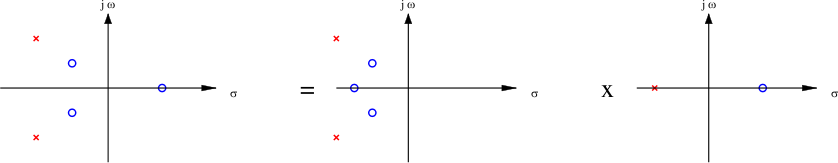
\includegraphics[width=12cm]{./images/nicht-minimalphasennetzwerk.png}\\
Nicht-Minimalphasennetzwerk (links) = Minimalphasennetzwerk (Mitte) · Allpass (rechts) \\
$H(s) = H_M(s) \cdot H_A(s)$

\subsection{Stabilitätsbestimmung am Pol-/Nullstellendiagramm}
\begin{tabular}{lcp{13cm}}
	asymptotisch stabil & = & alle Polstellen in der linken Halbebene (LHE) \\
	grenzstabil & = & Polstellen in der LHE und/oder auf der imaginären 
  Achse, Aber keine mehrfachen Pole auf der imaginären Achse \\
  instabil & = & Pol in RHE oder mehrfach Pole auf der imaginären Achse
\end{tabular}

\subsection{Bode-Diagramm \matlab{bode} \formelbuch{225-239}}
Siehe \formelbuch{225} für Beispiele\\
\begin{tabular}{ll}
	\parbox{7cm}{
		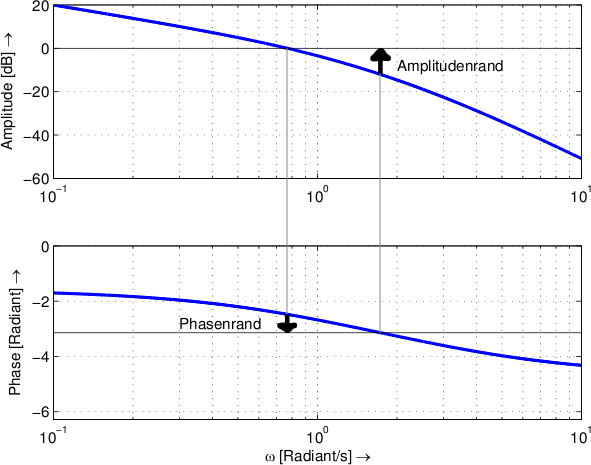
\includegraphics[width=7cm]{./images/bode-stabilitaet.png}
	}
	& \parbox{11cm}{
		\subsubsection{Definition}
		Das Bodediagramm besteht aus zwei Graphen, einer zeigt die Amplitude in
		doppelt-logarithmischer Form, der zweite zeigt die Phase in Grad und in
		linearer Form in Abhängigkeit der Frequenz dar.
		
		\subsubsection{Stabilitätsbestimmung \formelbuch{248-250} \matlab{margin,
		allmargin}}
		Der {\bf Amplitudenrand} ist der Abstand des
		Amplitudenganges zur 0~dB-Linie bei der Kreisfrequenz $\omega$, wo die Phase
		gleich $-\pi$ ist. \\
		
		Der {\bf Phasenrand} ist der Abstand das Phasenganges zur
		-$\pi$-Linie bei der Kreisfrequenz $\omega$, wo die Amplitude gleich 0~dB
		ist. \\
		
		Damit ein System stabil ist, m\"ussen Phasen- und Amplitudenrand
		$>0$ sein. Je gr\"osser diese sind, desto ``stabiler'' ist das System.
	}
\end{tabular}

\subsubsection{Vom Pol-/Nullstellendiagramm zum Bode-Diagramm \formelbuch{230}}
\begin{minipage}[b]{12cm}
  \[\boxed{ H(j\omega_0) = K \cdot \frac{(j\omega_0 - z_1)(j\omega_0-z_2)\ldots(j\omega_0-z_m)}
  {(j\omega_0-p_1)(j\omega_0-p_2)\ldots(j\omega_0-p_n)} = |H(j\omega_0)|\cdot \e^{j\varphi(\omega_0)}}\]

  \[ |H(j\omega_0)| = K \cdot \frac{\prod\limits_{i=1}^{m} A_{z_i}}{\prod\limits_{j=1}^{n} A_{p_i}}\]
  \[ \varphi(\omega_0) = \text{Phase von }K + \sum\limits_{i=1}^m \theta_{z_i} - \sum\limits_{j=1}^n \theta_{p_j}\]
\end{minipage}
\begin{minipage}[b]{7cm}
  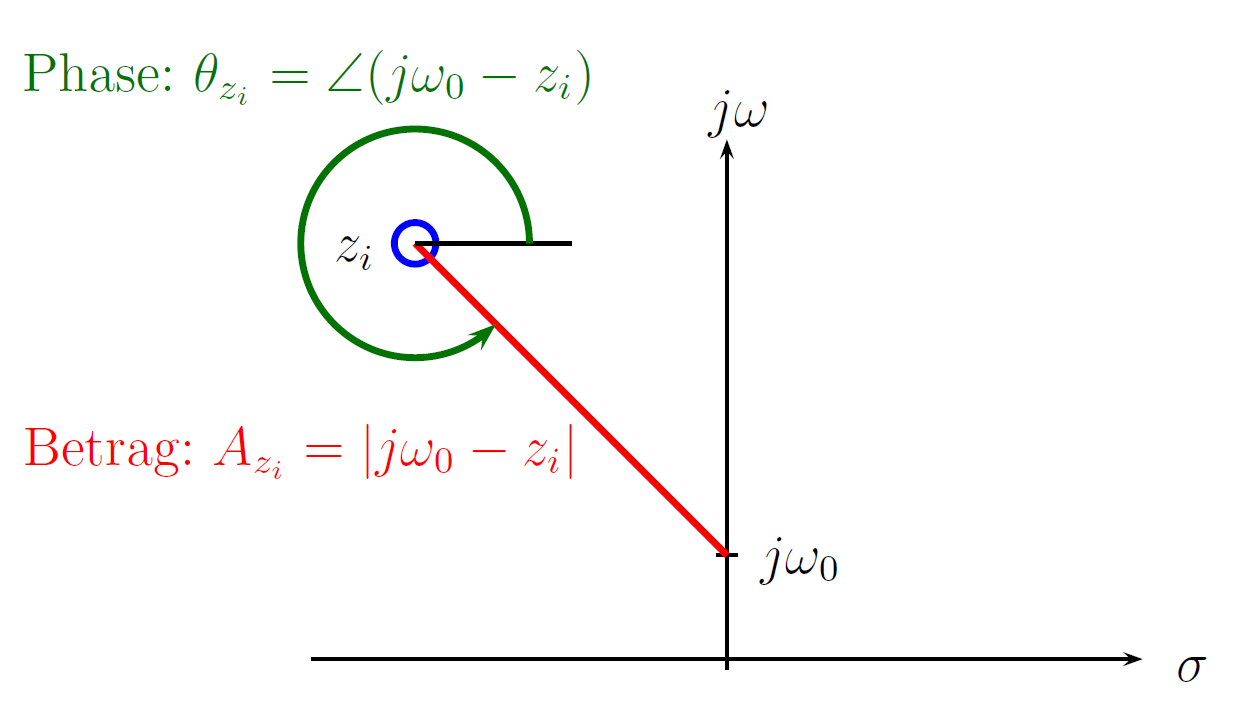
\includegraphics[width=7cm]{./images/PN_Diagramm.png}
\end{minipage}

\begin{minipage}{9cm}
\textbf{Grenzwerte:} \\

\begin{tabular}{|l|l|l|} \hline
\multirow{3}{*}{$\omega \rightarrow 0$} 
	& $\rightarrow \infty$ & Polstelle bei $\omega = 0$ \\
	& endlich & keine Pol- oder Nullstelle bei $\omega = 0$ \\ 
	& $\rightarrow 0$ & Nullstelle bei $\omega = 0$ \\ \hline
\multirow{3}{*}{$\omega \rightarrow \infty$} 
	& $\rightarrow \infty$ & mehr Null- als Polstellen \\
	& endlich & gleich viele Pol- und Nullstellen \\
	& $\rightarrow 0$ & mehr Pol- als Nullstellen \\ \hline
\end{tabular}
\end{minipage}
\begin{minipage}{9.5cm}
\begin{itemize}
  \item Pol auf Höhe $j\omega_x \Longrightarrow$ Überhöhung bei $\omega_x$
  \item Nullstelle auf Höhe $j\omega_x \Longrightarrow$ Dämpfung bei $\omega_x$
  \item $\frac{\prod{\text{Abstände NS zu 
        $\omega$}}}{\prod{\text{Abstände PS zu 
        $\omega$}}} > 1 \Longrightarrow$ Verstärkung
  \item $\frac{\prod{\text{Abstände NS zu 
        $\omega$}}}{\prod{\text{Abstände PS zu 
        $\omega$}}} < 1 \Longrightarrow$ Dämpfung
  \item Beim Durchlaufen eines Pols oder einer Nullstelle auf der $j\omega$-Achse, macht der Phasengang einen Sprung von $180^{\circ}$
\end{itemize}
\end{minipage}\\

\textbf{Regeln:}
\begin{itemize}
	\setlength{\itemsep}{-0.5em}
	\item reelle einfache Nullstellen ''knicken nach oben weg''
	\item reelle einfache Polstellen ''knicken nach unten weg''
	\item Pol-, Nullstellen auf der gleichen Stelle heben sich (theoretisch) auf
	\item konj. komplexe Nullstellen haben eine Senke
	\item konj. komplexe Polstellen haben eine Überhöhung
\end{itemize}

\newpage 
\begin{landscape}
\subsection{Approximation des Bode-Diagramms}
\renewcommand{\arraystretch}{1.5}
\begin{longtable}{|l|l|ll|ll|}
	\hline
		\textbf{Pole} & 
		\textbf{UTF} $H(s)$ &
		\multicolumn{2}{c}{\textbf{Amplitude} $|H(s)|$} & 
		\multicolumn{2}{|c|}{\textbf{Phase} $\angle(H(s))$}
	\\ \hline
		Keine, konstanter Faktor &
		$\alpha e^{j \beta}$ &
		\parbox[c][1cm]{1cm}{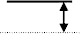
\includegraphics[width=1cm]{./bilder/bode-approx-konst.png}} &
		\, Konstant: $20 \log \alpha$ &
		\parbox[c][1cm]{1cm}{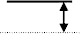
\includegraphics[width=1cm]{./bilder/bode-approx-konst.png}} &
		Konstant: $\beta$
	\\ \hline
		Pol im Ursprung &
		$\frac{\alpha}{s}$ &
		\parbox[c][1cm]{1cm}{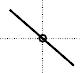
\includegraphics[width=1cm]{./bilder/bode-approx-ampl-tp-ord1.png}} & 
		\begin{tabular}{l}
			Lineare Steigung: $-20 dB/Dek.$ \\
			$0dB$ bei $\omega = \alpha$
		\end{tabular} &
		\parbox[c][1cm]{1cm}{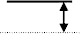
\includegraphics[width=1cm]{./bilder/bode-approx-konst.png}} & 
		Konstant: $-\frac{\pi}{2}$ 
	\\ \hline
		Nullstelle im Ursprung &
		$\alpha s$ &
		\parbox[c][1cm]{1cm}{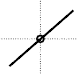
\includegraphics[width=1cm]{./bilder/bode-approx-ampl-hp-ord1.png}} & 
		\begin{tabular}{l}
			Lineare Steigung: $+20 dB/Dek.$ \\
			$0dB$ bei $\omega = \frac{1}{\alpha}$
		\end{tabular} &
		\parbox[c][1cm]{1cm}{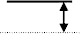
\includegraphics[width=1cm]{./bilder/bode-approx-konst.png}} &
		Konstant: $+\frac{\pi}{2}$
	\\ \hline	
		Reeller Pol &
		$\frac{1}{s + \alpha}$ &
		\parbox[c][1cm]{1cm}{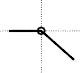
\includegraphics[width=1cm]{./bilder/bode-approx-ampl-4.png}} &
		\begin{tabular}{ll}
			$\omega < \alpha$: & Konstant $-20 \log \alpha$  \\
			$\omega > \alpha$: & $-20dB/Dek.$
		\end{tabular} &
		\parbox[c][1cm]{1cm}{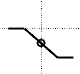
\includegraphics[width=1cm]{./bilder/bode-approx-phase-4.png}} &
		\begin{tabular}{ll}
			$\omega < \frac{\alpha}{10} $:	& Konstant $0$ \\
			$\omega > 10 \alpha$:		& Konstant $-\frac{\pi}{2}$
		\end{tabular}
	\\ \hline
		Reeller Pol &
		$\frac{\alpha}{s + \alpha}$ &
		\parbox[c][1cm]{1cm}{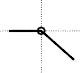
\includegraphics[width=1cm]{./bilder/bode-approx-ampl-4.png}} &
		\begin{tabular}{ll}
			$\omega < \alpha$: & Konstant $0dB$ \\
			$\omega > \alpha$: & $-20dB/Dek.$
		\end{tabular} &
		\parbox[c][1cm]{1cm}{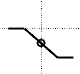
\includegraphics[width=1cm]{./bilder/bode-approx-phase-4.png}}	& 
		\begin{tabular}{ll}
			$\omega < \frac{\alpha}{10}$: & Konstant $0$ \\
			$\omega > 10 \alpha$: & Konstant $-\frac{\pi}{2}$
		\end{tabular}
	\\ \hline
		Reelle Nullstelle &
		$s + \alpha$ & 
		\parbox[c][1cm]{1cm}{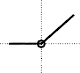
\includegraphics[width=1cm]{./bilder/bode-approx-ampl-5.png}} &
		\begin{tabular}{ll}
			$\omega < \alpha$: & Konstant $20 \log \alpha$ \\
			$\omega > \alpha$: & $+20dB/Dek.$
		\end{tabular} & 
		\parbox[c][1cm]{1cm}{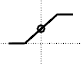
\includegraphics[width=1cm]{./bilder/bode-approx-phase-5.png}}	&
		\begin{tabular}{ll}
			$\omega < \frac{\alpha}{10}$: & Konstant $0$ \\
			$\omega > 10 \alpha$: & Konstant $+\frac{\pi}{2}$
		\end{tabular}
	\\ \hline	
		Reelle Nullstelle &
		$\frac{s + \alpha}{\alpha}$ &
		\parbox[c][1cm]{1cm}{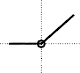
\includegraphics[width=1cm]{./bilder/bode-approx-ampl-5.png}} &
		\begin{tabular}{ll}
			$\omega < \alpha$: & Konstant $0dB$ \\
			$\omega > \alpha$: & $+20dB/Dek.$
		\end{tabular} &
		\parbox[c][1cm]{1cm}{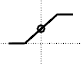
\includegraphics[width=1cm]{./bilder/bode-approx-phase-5.png}} &
		\begin{tabular}{ll}
			$\omega < \frac{\alpha}{10}$: & Konstant $0$ \\
			$\omega > 10 \alpha$: & Konstant $+\frac{\pi}{2}$
		\end{tabular}
	\\ \hline
		Konjugiert-komplexe Pole &
		$\frac{1}{s^2+s\frac{\omega_p}{q_p}+\omega_p^2}$ &
		\parbox[c][1cm]{1cm}{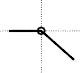
\includegraphics[width=1cm]{./bilder/bode-approx-ampl-6.png}} &
		\begin{tabular}{ll}
			$\omega < \omega_p$: 	& Konstant $-40 \log \omega_p$ \\
			$\omega > \omega_p$:	& $-40dB/Dek.$ \\
			Überhöhung: 			& $\frac{\omega_p}{2}$ bis $2\omega_p$ \\
			Maximum:				& $20 \log q_p$ bei $\omega = \omega_p$			
		\end{tabular} &
		\parbox[c][1cm]{1cm}{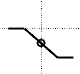
\includegraphics[width=1cm]{./bilder/bode-approx-phase-6.png}} &
		\begin{tabular}{ll}
			$\omega < \frac{\omega_p}{10^{\frac{1}{2q_p}}}$:	& Konstant $0$ \\
			$\omega > \omega_p 10^{\frac{1}{2q_p}}$:			& Konstant $-\pi$ \\
			$\omega = \omega_p$:								& $-\frac{\pi}{2}$
		\end{tabular}
	\\ \hline
		Konjugiert-komplexe Pole &
		$\frac{\omega_p^2}{s^2+s\frac{\omega_p}{q_p}+\omega_p^2}$ & 
		\parbox[c][1cm]{1cm}{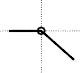
\includegraphics[width=1cm]{./bilder/bode-approx-ampl-6.png}} &
		\begin{tabular}{ll}
			$\omega < \omega_p$:	& Konstant $0dB$ \\
			$\omega > \omega_p$:	& $-40dB/Dek.$ \\
			Überhöhung:				& $\frac{\omega_p}{2}$ bis $2 \omega_p$ \\
			Maximum:				& $20 \log q_p$ bei $\omega = \omega_p$
		\end{tabular} &
		\parbox[c][1cm]{1cm}{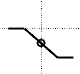
\includegraphics[width=1cm]{./bilder/bode-approx-phase-6.png}}	& 
		\begin{tabular}{ll}
			$\omega < \frac{\omega_p}{10^{\frac{1}{2q_p}}}$:	& Konstant $0$ \\
			$\omega > \omega_p 10^{\frac{1}{2q_p}}$:			& Konstant $-\pi$ \\
			$\omega = \omega_p$:								& $-\frac{\pi}{2}$
		\end{tabular}
	\\ \hline	
		Konjugiert-komplexe Nullstellen &
		$s^2+s\frac{\omega_z}{q_z}+\omega_z^2$ &
		\multicolumn{4}{l|}{
			Analog zu den Konjugiert-komplexen Polen jedoch gespiegelt an der $0dB$- / $0$-Grad-Linie.
		}
	\\
		&
		$\frac{s^2+s\frac{\omega_z}{q_z}+\omega_z^2}{\omega_z^2}$ &
		\multicolumn{4}{l|}{}
	\\ \hline
		\multicolumn{6}{|p{21cm}|}{
			Serieschaltung von Systemen erfolgt durch \textbf{Superposition} der einzelnen Bode-Diagramme 
			(Multiplikation von UTFs entspricht Addition im	dB-Bereich).
		}
	\\ \hline
\end{longtable}
\renewcommand{\arraystretch}{\arraystretchOriginal}
\end{landscape}
\renewcommand{\arraystretch}{1}

%\textbf{Werte für $q_p$ bzw. $q_z$}\\
%\renewcommand{\arraystretch}{1.5}
%\begin{tabular}{|r|r|r||r|r|r||r|r|r||r|r|r||r|r|r|}
%\hline
%\multicolumn{1}{|l|}{$q$} & \multicolumn{1}{l|}{$10^{\frac{1}{2 q_p}}$} & 
%\multicolumn{1}{l||}{$\frac{1}{10^{\frac{1}{2 q_p}}}$} &
%\multicolumn{1}{l|}{$q$} & \multicolumn{1}{l|}{$10^{\frac{1}{2 q_p}}$} &
%\multicolumn{1}{l||}{$\frac{1}{10^{\frac{1}{2 q_p}}}$} &
%\multicolumn{1}{l|}{$q$} & \multicolumn{1}{l|}{$10^{\frac{1}{2 q_p}}$} & \multicolumn{1}{l||}{$\frac{1}{10^{\frac{1}{2 q_p}}}$} & \multicolumn{1}{l|}{$q$} & \multicolumn{1}{l|}{$10^{\frac{1}{2 q_p}}$} & \multicolumn{1}{l||}{$\frac{1}{10^{\frac{1}{2 q_p}}}$} & \multicolumn{1}{l|}{$q$} & \multicolumn{1}{l|}{$10^{\frac{1}{2 q_p}}$} & \multicolumn{1}{l|}{$\frac{1}{10^{\frac{1}{2 q_p}}}$} \\ \hline
%\hline
%1 & 3.162 & 0.316 & 5 & 1.259 & 0.794 & 9 & 1.136 & 0.880 & 13 & 1.093 & 0.915 & 17 & 1.070 & 0.935 \\ \hline
%2 & 1.778 & 0.562 & 6 & 1.212 & 0.825 & 10 & 1.122 & 0.891 & 14 & 1.086 & 0.921 & 18 & 1.066 & 0.938 \\ \hline
%3 & 1.468 & 0.681 & 7 & 1.179 & 0.848 & 11 & 1.110 & 0.901 & 15 & 1.080 & 0.926 & 19 & 1.062 & 0.941 \\ \hline
%4 & 1.334 & 0.750 & 8 & 1.155 & 0.866 & 12 & 1.101 & 0.909 & 16 & 1.075 & 0.931 & 20 & 1.059 & 0.944 \\ \hline
%\end{tabular}
%\renewcommand{\arraystretch}{1}\\


\subsection{Ortskurve (Nyquist-Diagramm) \matlab{nyquist} \formelbuch{240-247}}
\begin{tabular}{ll}
	\parbox{5cm}{
		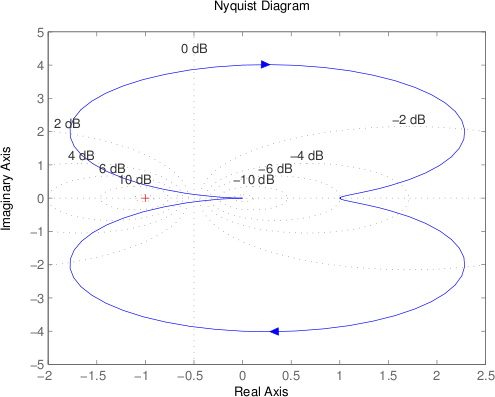
\includegraphics[width=5cm]{./images/nyquist.png}
    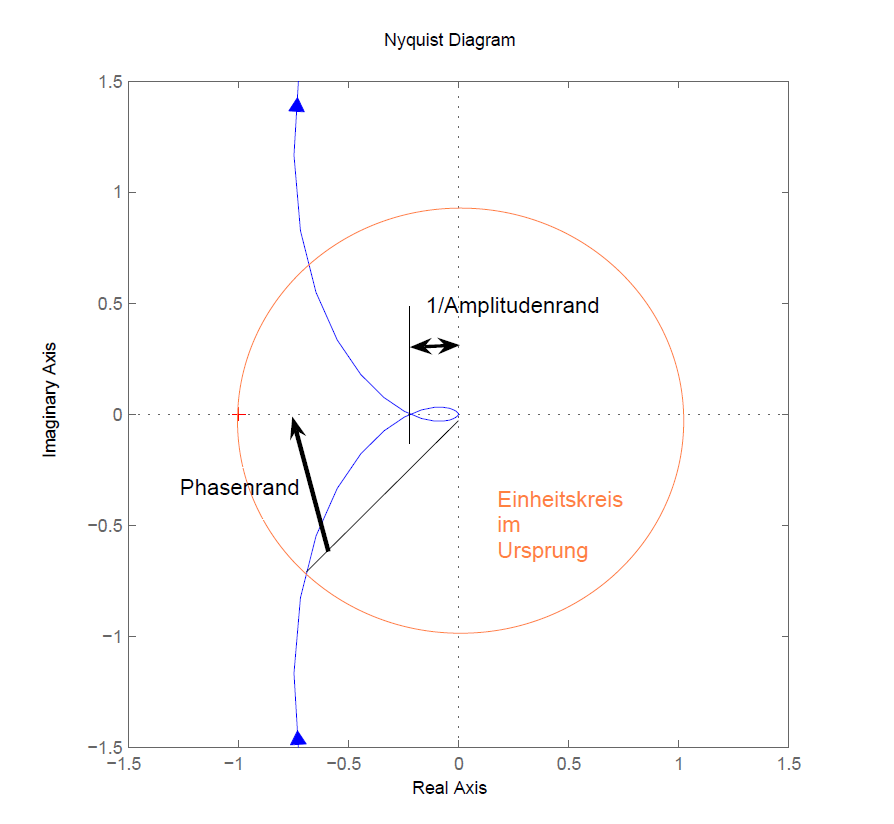
\includegraphics[width=5cm]{./images/nyquist_stab.png}
	}
	& \parbox{13cm}{
		\subsubsection{Definition}
		Im Gegensatz zum Bode-Diagramm wird beim Nyquist-Diagramm Betrag und Phase in
		einem einzigen Diagramm dargestellt, nämlich indem man den Real- und
		Imaginärteil des Ausgabewertes direkt in die komplexe Zahlenebene zeichnet.
		
		\subsubsection{Stabilitätsbestimmung \formelbuch{245-247}}
		Ist der {\bf offene} Regelkreis $H(s)$ {\bf asymptotisch
		stabil}\index{asymptotisch stabil}, so ist der {\bf geschlossene}
		Regelkreis $1+H(s)=D(s)+N(s)$ asymptotisch stabil, wenn die {\bf
		Ortskurve} des {\bf offenen} Regelkreises den kritischen Punkt
		(-1,$j0$) weder umkreist noch durchl\"auft.
	}

\end{tabular}


\subsection{Nichols-Diagramm \matlab{nichols}}
\begin{tabular}{ll}
	\parbox{5cm}{
		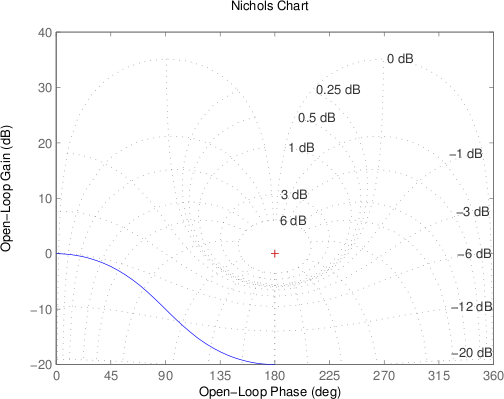
\includegraphics[width=5cm]{./images/nichols.png}
    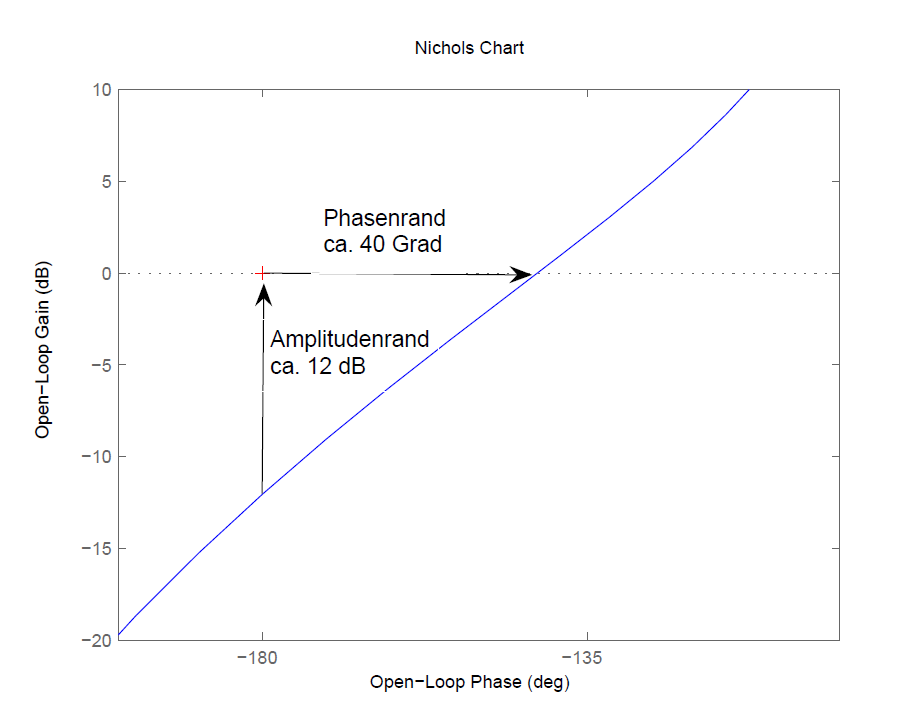
\includegraphics[width=5cm]{./images/nichols_stab.png}
	}
	& \parbox{11cm}{
		\subsubsection{Definition}
		Das Nichols Diagramm (auch Amplituden-Phasen-Diagramm) ist die Darstellung des
		Absolutbetrages (Verstärkung, logarithmisch) in Abhängigkeit der Phase. Das Nichols Diagramm ist zur
		Bestimmung der Stabilität in rückgekoppelten Systemen verwendbar.
    
    \subsubsection{Stabilitätsbestimmung}
    Beim Nichols Diagramm lassen sich Amplitudenrand und Phasenrand am einfachsten aus dem Diagramm lesen.
	}
\end{tabular}

\subsection{Phasen-, und Gruppenlaufzeit \formelbuch{182-186}}
  \begin{tabular}{|l|l|p{10cm}|}
    \hline
      & \textbf{Formel} & \textbf{Definition}\\
    \hline
      Phasenlaufzeit\formelbuch{182} &
      $ \tau_P(\omega) = \dfrac{-\varphi(\omega)}{\omega}$ &
      Die Phasenlaufzeit ist nur für \textbf{reine Sinusschwingungen} exakt bestimmbar. 
      Mit einer Phasenlaufzeit wird das Ausgangssignal wird gegenüber dem Eingangsignal verzögert. \\
    \hline
      Gruppenlaufzeit\formelbuch{183} &
      $\tau_g(\omega) = \dfrac{-\mathrm{d}\varphi(\omega)}{\mathrm{d}\omega}$ &
      Die Gruppenlaufzeit gilt für Signale mit mehreren Frequenzanteilen. Die Gruppenlaufzeit
      kann als \textbf{Laufzeit eines Signals} interpretiert werden. \\
    \hline
  \end{tabular}
  
\subsection{Bestimmung der UTF aus dem Frequenzgang \formelbuch{292}}
  \begin{tabular}{p{6cm}p{12cm}}
    \vspace{-1.5\topsep}
    $\dfrac{N(s)}{D(s)} \cdot \dfrac{N(-s)}{D(-s)} = \left.|H(j\omega)|^2\right|_{\omega^2=-s^2}$ &
    Aus Stabilitätsgründen muss $D(s)$ ein Hurwitz-Polynom sein.
  \end{tabular}








